\section{Estimating the model using a Gibbs Sampler} \label{sec:estimation}
While the simulation yields results, it used values that originally came from the Metropolis-Hastings Algorithm \citep[Appendix, p. 2]{agarwal_organic_2015}. To estimate the factors that drive the click-through rate and the orders, we implemented a Gibbs sampler. The original model runs 40,000 iterations as burn-in and 80,000 iterations in total.\\
A Bayesian model needs appropriate priors and a likelihood. The priors used in the model have been introduced as the distributions in section \ref{sec:intro}. The likelihood is a combined Bernoulli likelihood for both $U^{CTR}_{kt}$ and $U^{CONV}_{kt}$ \citep[Appendix, p. 2]{agarwal_organic_2015}. Yet, this hierarchical model is a triangular system, meaning it involves recursive elements which then become directed cycles. This imposed a problem when following the approach. The different steps have been summarized in table \ref{table:MCMC}.

\begin{longtable}{| p{0.2cm} | p{1.5cm} | p{4.5cm} | p{4.5cm} |}
    \hline
    &\textbf{Method} & \textbf{Main Focus} & \textbf{Solution}\\
    \hline \hline
    1 & JAGS & A basic implementation of the model. &\\
    &&&\\
    && The paper's likelihood is a combined likelihood for both $U^{CTR}_{kt}$ and $U^{CONV}_{kt}$ and is dependent on itself. It does not match the input required by JAGS. & It was replaced by a simple Bernoulli likelihood using \texttt{dbern()}.\\
    & & When fully specified, the model seems to be recursive, it involves directed cycles, a "simultaneous model" as also stated by the authors \citep[p. 19]{agarwal_organic_2015}. In JAGS however, directed cycles are forbidden \citep[p. 15]{JAGS}. It returned a compilation error and "possible directed cycle involving deltaTildeAlpha". The syntactically correct model \texttt{JAGS\_attempt.R} can be found in the apppendix.
    & In contrast to JAGS, BUGS allows directed cycles at a user's own risk. BUGS was therefore installed and run by \texttt{R2OpenBGUS}.\\
    \hline
    2 & BUGS & Though similar to JAGS, BUGS uses a slightly different syntax and generally offered fewer logical elements such as functions or conditional statements, e.g.: &\\
    &&&\\
    && - \texttt{\%*\%} & - matrix multiplication in loops instead of \texttt{\%*\%}\\
    && - \texttt{if} statements & - replaced \texttt{if} by \texttt{step()}\\
    && - \texttt{dbern()} throws an error & - replaced by \texttt{dnorm()} for the sake of simplicity\\
    && &\\
    \hline
    && In the end, BUGS reported a stack overflow which "can occur if there is a recursive definition of a logical node", so a simultaneous model. The syntactically correct model \texttt{BUGS\_attempt.R} can be found in the appendix. & An alternative to BUGS is the package \texttt{bayesm}. The package and the accompanying book \citep{rossibook} seem to match our model and allow for simultaneous models as well. \\
    \hline
    3 & \texttt{bayesm} & Overall, the authors seemed to have followed Rossi et al.'s approach. In particular, the function \texttt{rhierMnlRwMixture} is quite similar to the model, but would need adjustments to mirror the model. & Based on the package and its functions, an MCMC could very well be defined by us as well. After all, the Metropolis only seems to be "another algorithm".\\
    \hline
    4 & Metropolis Hastings by hand & The appended file \texttt{Metropolis\_Hastings.R} defined all necessary steps to run an MCMC by hand. It follows the appendix of the original paper. Though it encountered further dimension problems and notation issues, it was interpreted in a way that it matched dimension-wise. Unfortunately, the estimated values grow to $\infty$ after 5-7 big iterations, depending on the seed. We strongly suspect this is due to an incorrect use of the inverse, be it a notation problem or a problem in the code. See the code for more details. & To have a simple running model, JAGS was employed again.\\
    \hline
    5 & JAGS & The last JAGS model implements the main four equations from equations \ref{eq:mainlinear} and \ref{eq:endogeneous} and assumes normally distributed parameters. The $\epsilon$ error terms have been taken from the simulation in \ref{sec:simulation}. Parts of it can be seen below. The full model is denoted as \texttt{JAGS\_running.R}. & \\
    \hline
\caption{A short overview to the approaches to using a Markov Chain Monte Carlo algorithm or a Gibbs sampler for this model.}
\label{table:MCMC} 
\end{longtable}

\newpage
\begin{lstlisting}[caption={Estimating the model with a very basic JAGS version}]
modelString = "
model {
for (j in 1:N){
for (i in 1:M){

ctr[i, j] ~ dnorm(p[i,j], 1)
p[i, j] <- exp( z[i, j] ) / ( 1 + exp( z[i, j] ) )
z[i, j] <- (-4.22 + theta0) + (-1.42 + theta1) * adpos_eq[i, j] + random_thetas[3, i] * orgcomp_eq[i, j] 
+ random_thetas[4, i] * sponsored_comp[i, j] + theta4 * organic[i, j]
+ theta5 * lqscore[i, j] + theta6 * i + theta_error[i, j] 

conv[i, j] ~ dnorm(r[i, j], 1)
r[i, j] <- exp(q[i, j]) / (1 + exp(q[i, j]))
q[i,j] <- (-2.75 + beta0) + (0.81 + beta1) * adpos_eq[i, j] + random_betas[3, i] * orgcomp_eq[i, j] + 
random_betas[4, i] * sponsored_comp[i, j] + beta4 * organic[i, j] + 
beta5 * lqscore[i, j] + beta6 * i + beta_error[i, j]

adpos_eq[i, j] <- exp(random_gammas[1, i] + random_gammas[2, i] * log(bid[i, j]) + gamma2 * lqscore[i, j] +
                   gamma3 * i + gamma_error[i, j])

orgcomp_eq[i, j] <- random_alphas[1, i] + random_alphas[2, i] * iv_organic[i, j] +
                     alpha2 * i + alpha_error[i, j]

}
}
gamma2 <- -0.049
gamma3 <- -0.002

alpha2 <- -0.004

theta0 ~ dnorm(0, 0.55)
theta1 ~ dnorm(0, 0.18)
theta4 <- -0.2
theta5 <- 0.3 
theta6 <- -0.01

beta0 ~ dnorm(0, 0.68)
beta1 ~ dnorm(0, 0.28)
beta4 <- 0.17
beta5 <- -0.01
beta6 <- -0.01
}
"
writeLines( modelString, con="TEMPmodel.txt")

jags <- jags.model('TEMPmodel.txt',
                   data = list('N' = num_days,
                               'M' = num_keywords,
                               'adpos' = adpos,
                               'ctr' = CTR_estimate,
                               'conv' = CONV_estimate,
                               'bid' = bid,
                               'iv_organic' = iv_organic,
                               'orgcomp' = organic_comp,
                               'organic' = organic,
                               'sponsored_comp' = sponsored_comp,
                               'lqscore' = lqscore,
                               'theta_error' = theta_error,
                               'beta_error' = beta_error,
                               'random_betas' = random_betas,
                               'random_thetas' = random_thetas,
                               'random_gammas' = random_gammas,
                               'random_alphas' = random_alphas,
                               'gamma_error' = gamma_error,
                               'alpha_error' = alpha_error),
                   n.chains = 4,
                   n.adapt = 1000)

update(jags, 1000)

\end{lstlisting}

Although we ran into some calculation issues with our more complicated model, we were able to achieve results using a simplified version. In this version, 1000 adaptations were followed by a 1000 burn-in period. The plots here show the previous values for CTR and CONV that were calculated by our data simulation, the summary statistics-specified CTR and CONV, and the new values for these two rates calculated by JAGS.

\begin{figure}[!h]
    \centering
    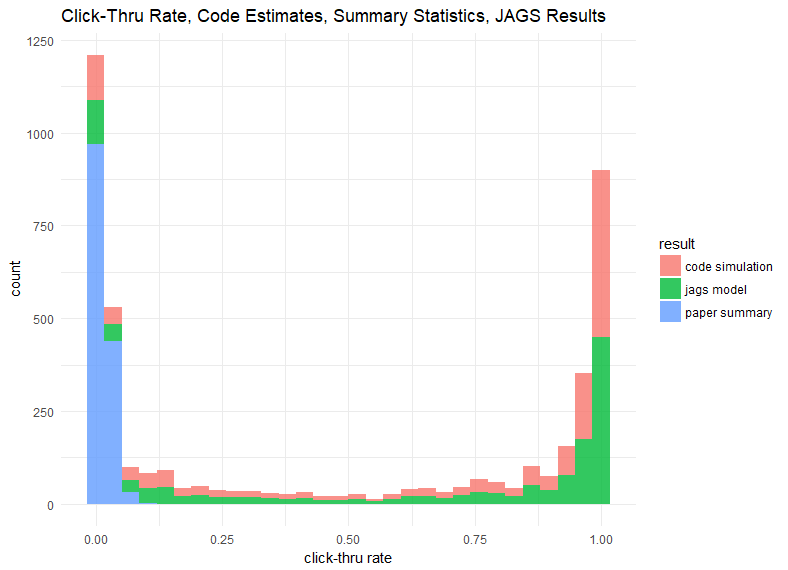
\includegraphics[scale = 0.55]{ctr_jags_plot.png}
    \caption{Count of simulated and summary statistic-based CTR estimates}
    \label{fig:ctr-jags}
\end{figure}

 The distribution of the JAGS-generated CTR values is shown as somewhere between the data-simulated values and those from the summary statistics - this is displayed in figure \ref{fig:conv-jags}. As seen in figure \ref{fig:ctr-jags}, the spread of the conversation rates also follows this pattern.

\begin{figure}[!h]
    \centering
    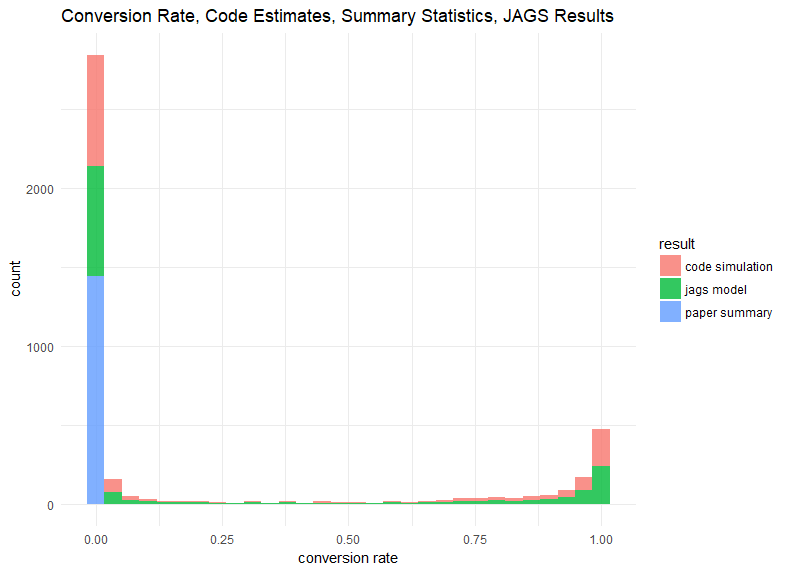
\includegraphics[scale = 0.55]{conv_jags_plot.png}
    \caption{Count of simulated and summary statistic-based CTR estimates}
    \label{fig:conv-jags}
\end{figure}

As we see in the the trace plots of theta0 and theta1 (figure \ref{fig:trace-theta0}), the distribution of the chain is relatively normal and the trajectory is stable over time. As we are expecting to see normal distributions, this is a good indicator that things are working properly \citep{MCMCDiagnostic}.

\begin{figure}[!h]
    \centering
    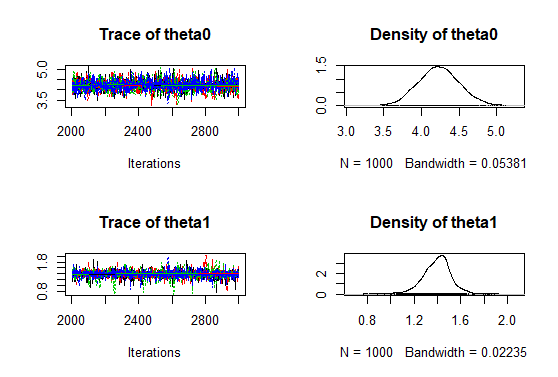
\includegraphics[scale = 0.65]{theta0_trace.png}
    \caption{Trace plot of Theta0 and Theta1 from JAGS model}
    \label{fig:trace-theta0}
\end{figure}

Looking at figure \ref{fig:gelman-theta0}, the Gelman plots for theta0 and theta1, we see that the appear to be well-disbursed throughout the sampling period. This indicates that our chains are relatively similar to each other, at least in terms of values for theta0.

\begin{figure}[!h]
    \centering
    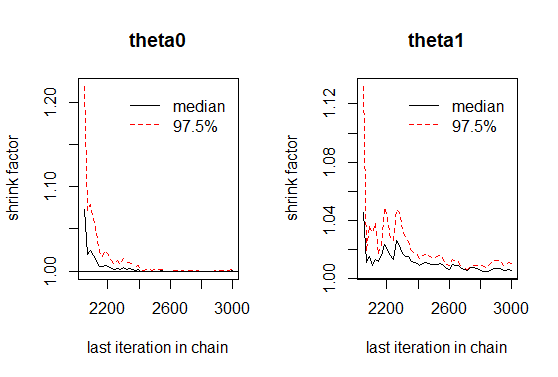
\includegraphics[scale = 0.65]{theta0_gelman.png}
    \caption{Gelman plots of Theta0 and Theta1}
    \label{fig:gelman-theta0}
\end{figure}